\documentclass{article}
\usepackage{graphicx} % Required for inserting images

\title{CTA200H Assignment 3 Writeup}
\author{Alyssa Atkinson }
\date{May 9th 2023}

\begin{document}


\maketitle{}

\section{Question 1}

In this question, the goal was to iterate the equation $z_{i + 1} = z_i^2 + c$ over the complex plane $-2 < x < 2$ and $-2 < y < 2$ to create images of the Mandelbrot set.  To do this, a function in a  a separate file called iterate was defined which iterated the equation over each point in the complex plane. 

\hfill \break
To visualize the results of the iteration, points which diverged(went to infinity) were coloured to be blue while points that converged were coloured to be red. An image of the plane showing which points converged vs diverged was created using matplotlib:

\begin{center}
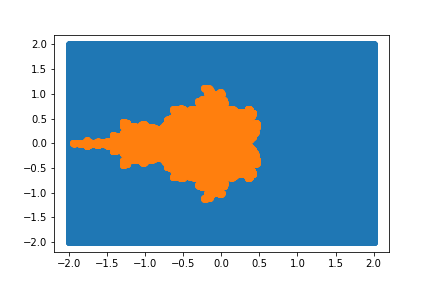
\includegraphics[width=100mm]{image1.png}
\end{center}

\\\caption{Figure 1: Mandelbrot set. Orange points converge while blue points diverge.}
  \label{fig:fig1}


\hfill \break
A second image was created with colour as a third variable, indicating the index at which a given point diverged: 
\begin{center}
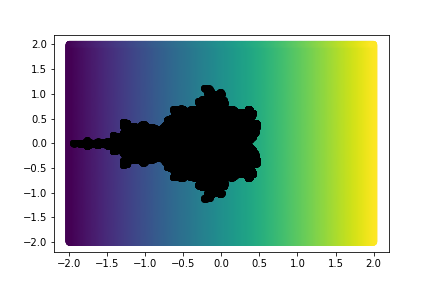
\includegraphics[width=100mm]{image2.png}
\end{center}
\\\caption{Figure 2: Mandelbrot set where black points converge and the points that diverge are coloured by a colourscale which indicates when they diverged .}
  \label{fig:fig2}


\section{Question 2}

{In this question, the goal was to solve the differential equations related to atmospheric conditions defined by Edward Lorenz, and recreate his numerical analysis:  }

\begin{eqnarray}
\dot X &=& -\sigma(X-Y)\\
\dot Y &=& rX -Y - XZ\\
\dot Z &=& -bZ + XY
\end{eqnarray}

\hfill \break

First, using the same initial conditons $W_0=[0., 1., 0.]$ and parameters [$\sigma, r, b$] = [10., 28, 8./3.] used by Lorenz, the numpy function  solve\_ivp was used to solve this system. The timespan of integration used was 0 to 60 seconds. The solution to the Lorenz equations were plotted to recreate the original plots in Lorenz's paper: 

\begin{center}
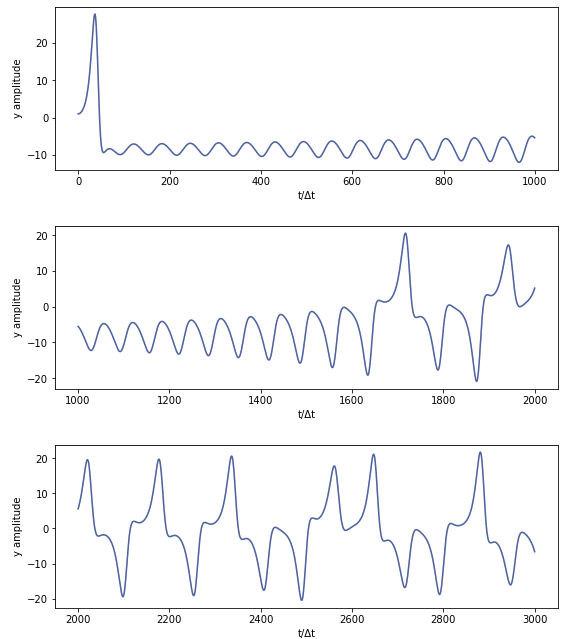
\includegraphics[width=70mm]{fig1.png}
\\\caption{Figure 3: Recreation of Lorenz's Figure 1 Using solve_\ivp .}
  \label{fig:fig3}
  

\hfill \break

This method was also used to recreate Figure 2 in Lorenz's paper:

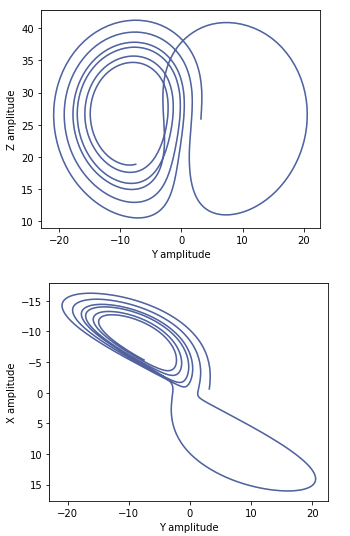
\includegraphics[width=50mm]{fig2.png}

\\\caption{Figure 4: Recreation of Lorenz's Figure 2 Using solve_\ivp .}
  \label{fig:fig2}
  
\end{center}
\hfill \break



Next, the initial conditions were changed to be $W_0$, say $W'_0 = W_0+[0., 1.e-8, 0] = [0., 1.00000001, 0.]$. solve_\ivp was once again used to solve the equation. Then, the difference between each point in the two solutions wad calculated in a loop. Using this, in combination with np.linalg.norm,  the distance between the two solutions was computed. The following is a plot of this distance vs time: 


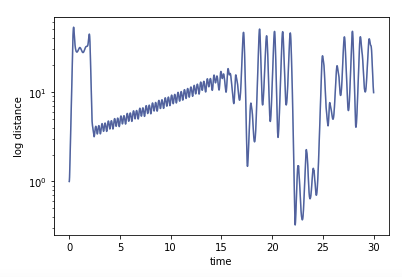
\includegraphics[width=80mm]{fig 5.png}
\\\caption{Figure 5: Distance vs time of the two solutions (with distance log-scaled.  .}
  \label{fig:fig5}

\section{References}
Lorenz, E. N., 1963: Deterministic Nonperiodic Flow. J. Atmos. Sci., 20, 130–141, https://doi.org/10.1175/1520-0469(1963)020<0130:DNF>2.0.CO;2.


\end{document}
